%----------------------------------------------------------------------------------------
%	CHAPTER 6
%----------------------------------------------------------------------------------------
\chapterimage{ChapterImages/chapter6.png} % Chapter heading image

\chapter{Shell Programming II}
\label{ch:shell2}

This chapter builds directly on Chapter~\ref{ch:shell1}: with variables, conditionals, and test operators already in hand, the missing piece for writing genuinely useful scripts is \textbf{repetition} -- running the same commands over a list of items, or until some condition changes. That is what loops give you.

\section{Introduction to Loops}
Loops let you repeat commands in a script, which is useful for handling repetitive tasks efficiently. Instead of writing the same code many times, a loop runs it automatically over a list or for as long as a condition holds.

\subsection{Why Use Loops}
In system administration and scripting, loops give you three things at once:
\begin{itemize}
    \item \textbf{Efficiency:} automate repetitive work, such as processing many files or counting through a range of numbers.
    \item \textbf{Readability:} keep scripts short and easy to maintain, instead of repeating near-identical lines.
    \item \textbf{Common uses:} repeating an action (e.g.\ printing messages), processing data (e.g.\ reading lines from a file), or waiting for a condition (e.g.\ until a counter reaches zero).
\end{itemize}
Without loops, you would need to write the same commands multiple times, making scripts longer, harder to maintain, and more prone to errors.

\subsection{Types of Loops in Bash}
Bash provides three primary loop structures, each suited to a different scenario:

\begin{table}[h!]
\centering
\small
\renewcommand{\arraystretch}{1.3}
\begin{tabular}{|>{\centering\arraybackslash}p{3cm}|>{\raggedright\arraybackslash}p{9cm}|}
\hline
\textbf{Loop Type} & \textbf{Best Used When} \\ \hline
\texttt{for} & You have a specific list of items to process \\ \hline
\texttt{while} & You want to continue \emph{while} a condition remains true \\ \hline
\texttt{until} & You want to continue \emph{until} a condition becomes true \\ \hline
\end{tabular}
\caption{Common Loop Types in Shell Scripting}
\label{tab:loop-types}
\end{table}

\subsection{Loop Execution Flow}
Regardless of which loop you use, the same four steps repeat in a cycle, shown in Figure~\ref{fig:loop-flow}:
\begin{enumerate}
    \item \textbf{Initialization:} set up any variables the loop depends on.
    \item \textbf{Condition Check:} evaluate whether to continue.
    \item \textbf{Body Execution:} run the commands inside the loop.
    \item \textbf{Update:} modify the loop variable, then return to step 2.
\end{enumerate}

\begin{figure}[h]
    \centering
    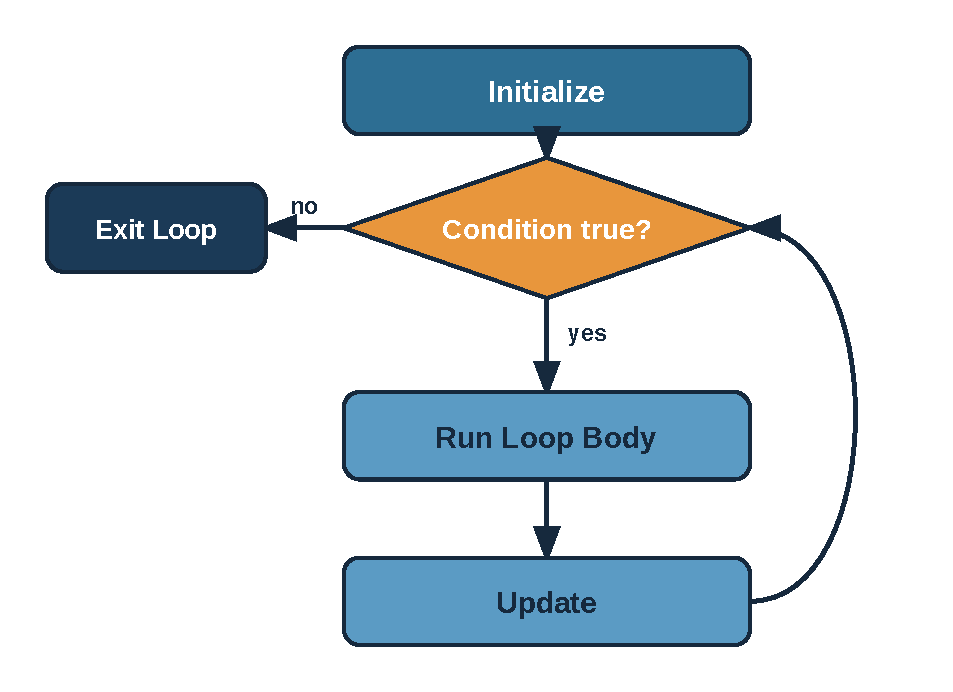
\includegraphics[width=0.75\textwidth]{Images/Chapter6/loop-flow.pdf}
    \caption{The general execution flow shared by \texttt{for}, \texttt{while}, and \texttt{until} loops.}
    \label{fig:loop-flow}
\end{figure}

\section{The \texttt{for} Loop}
The \texttt{for} loop is great for going through a fixed list of items, such as numbers or words. It assigns each item to a variable one at a time and runs the loop body once per item.

\subsection{Basic Syntax and Explanation}
\begin{lstlisting}[language=Terminal]
#!/bin/bash
for variable in list; do
    # Commands to run for each item
done
\end{lstlisting}
\begin{itemize}
    \item \textbf{variable}: holds the current item from the list on each pass.
    \item \textbf{list}: the items to loop through (e.g.\ words or numbers).
    \item \textbf{do ... done}: the block of commands that runs on every pass.
\end{itemize}
This loop runs exactly once per item in the list -- there is no separate condition check like in \texttt{while}/\texttt{until}.

\subsection{Creating Lists for Loops}
You can build the list in several simple ways:
\begin{itemize}
    \item Direct words: \texttt{apple banana orange}
    \item Numbers with brace expansion: \texttt{\{1..5\}} (expands to \texttt{1 2 3 4 5})
    \item From a command's output: \texttt{\$(ls *.txt)} (lists all \texttt{.txt} files)
\end{itemize}

\subsection{Practical Basic Examples}

\textbf{Example 1: Print Fruits}\\
This loops through a list of fruits and prints a message for each.
\begin{lstlisting}[language=Terminal]
#!/bin/bash
for fruit in apple banana orange; do
    echo "I like $fruit"
done
\end{lstlisting}
\textbf{Explanation:} the list is \texttt{apple banana orange}; for each one, the script echoes \texttt{"I like [fruit]"}.
\begin{lstlisting}[language=Terminal]
I like apple
I like banana
I like orange
\end{lstlisting}

\textbf{Example 2: Count Numbers}\\
This uses brace expansion for numbers.
\begin{lstlisting}[language=Terminal]
#!/bin/bash
for num in {1..5}; do
    echo "Number: $num"
done
\end{lstlisting}
\textbf{Explanation:} \texttt{\{1..5\}} creates the list \texttt{1 2 3 4 5}, and the loop prints each number.
\begin{lstlisting}[language=Terminal]
Number: 1
Number: 2
Number: 3
Number: 4
Number: 5
\end{lstlisting}
Useful for fixed ranges known ahead of time.

\subsection{C-style \texttt{for} Loop}
Bash also supports a C-style \texttt{for} loop syntax, which is convenient for numeric iteration:
\begin{lstlisting}[language=Terminal]
#!/bin/bash
for ((initialization; condition; update)); do
    # commands
done
\end{lstlisting}

\textbf{Example:}
\begin{lstlisting}[language=Terminal]
#!/bin/bash
for ((i=0; i<10; i++)); do
    echo "Iteration: $i"
done

# With step increments
for ((i=0; i<=20; i+=5)); do
    echo "Value: $i"
done
\end{lstlisting}

\section{The \texttt{while} Loop}
The \texttt{while} loop repeats commands for as long as a condition is true. It's the right choice when you don't know in advance how many times the loop needs to run.

\subsection{Basic Syntax and Explanation}
\begin{lstlisting}[language=Terminal]
#!/bin/bash
while [ condition ]; do
    # Commands
done
\end{lstlisting}
\begin{itemize}
    \item \texttt{[ condition ]} is checked before each pass (e.g.\ \texttt{[ \$counter -gt 0 ]}).
    \item If it is true (exit status \texttt{0}), the loop body runs; otherwise, the loop stops.
    \item Remember to update the tested variable inside the loop body -- forgetting to do so causes an infinite loop.
\end{itemize}

\subsection{Reading Files with \texttt{while}}
A common use of \texttt{while} is reading a file line by line:
\begin{lstlisting}[language=Terminal]
#!/bin/bash
while read line; do
    echo "$line"
done < file.txt
\end{lstlisting}
This reads each line of \texttt{file.txt} into \texttt{\$line} and processes it, one line per pass.

\subsection{Practical Basic Examples}

\textbf{Example 1: Countdown}\\
This counts down from 5 to 1.
\begin{lstlisting}[language=Terminal]
#!/bin/bash
counter=5
while [ $counter -gt 0 ]; do
    echo "Countdown: $counter"
    ((counter--))  # Decrease counter by 1
done
\end{lstlisting}
\textbf{Explanation:} starts with \texttt{counter=5}; the condition is ``while \texttt{counter > 0}''; the script prints and decreases the counter on every pass.
\begin{lstlisting}[language=Terminal]
Countdown: 5
Countdown: 4
Countdown: 3
Countdown: 2
Countdown: 1
\end{lstlisting}
This demonstrates both condition checking and updating in the same loop.

\textbf{Example 2: Sum Numbers}\\
This sums the numbers from 1 to 5.
\begin{lstlisting}[language=Terminal]
#!/bin/bash
sum=0
num=1
while [ $num -le 5 ]; do
    sum=$((sum + num))
    ((num++))
done
echo "Sum: $sum"
\end{lstlisting}
\textbf{Explanation:} initializes \texttt{sum=0} and \texttt{num=1}, then adds \texttt{num} to \texttt{sum} while \texttt{num <= 5}, increasing \texttt{num} each pass. Output: \texttt{Sum: 15}. This shows how arithmetic accumulates across loop iterations.

\section{The \texttt{until} Loop}
The \texttt{until} loop is the mirror image of \texttt{while}: it keeps running \emph{as long as} its condition is false, and stops as soon as the condition becomes true.

\subsection{Basic Syntax and Explanation}
\begin{lstlisting}[language=Terminal]
#!/bin/bash
until [ condition ]; do
    # Commands
done
\end{lstlisting}
\begin{itemize}
    \item The loop body runs while the condition is false (non-zero exit status).
    \item \texttt{until [ condition ]} is equivalent to \texttt{while ! [ condition ]}.
\end{itemize}

\subsection{Comparison with \texttt{while}}
The two loops below behave identically -- they are just two ways of expressing the same stopping point:
\begin{lstlisting}[language=Terminal]
while [ $x -lt 5 ]; do ... done    # keep going while x < 5
until  [ $x -ge 5 ]; do ... done   # keep going until x >= 5
\end{lstlisting}
Use \texttt{until} when it is more natural to think in terms of ``stop once this happens'' rather than ``keep going while this holds''.

\subsection{Practical Basic Examples}

\textbf{Example 1: Count Up}\\
This counts from 1 to 5.
\begin{lstlisting}[language=Terminal]
#!/bin/bash
counter=1
until [ $counter -gt 5 ]; do
    echo "Counter: $counter"
    ((counter++))
done
\end{lstlisting}
\textbf{Explanation:} starts at \texttt{1}; runs until \texttt{counter > 5} (i.e.\ while \texttt{counter <= 5}); prints and increases the counter each pass.
\begin{lstlisting}[language=Terminal]
Counter: 1
Counter: 2
Counter: 3
Counter: 4
Counter: 5
\end{lstlisting}

\textbf{Example 2: Wait for a Number}\\
This waits until a variable reaches 3.
\begin{lstlisting}[language=Terminal]
#!/bin/bash
attempt=0
until [ $attempt -eq 3 ]; do
    ((attempt++))
    echo "Attempt: $attempt"
done
\end{lstlisting}
\textbf{Explanation:} increases \texttt{attempt} until it equals \texttt{3}.
\begin{lstlisting}[language=Terminal]
Attempt: 1
Attempt: 2
Attempt: 3
\end{lstlisting}
A simple pattern for simulating retries.

\section{Loop Control Statements}
These statements change how a loop runs -- stopping it early or skipping a step -- and work inside any of the three loop types.

\subsection{The \texttt{break} Statement}
\texttt{break} exits the loop immediately.
\begin{lstlisting}[language=Terminal]
#!/bin/bash
for num in {1..5}; do
    if [ $num -eq 3 ]; then
        break  # Stop at 3
    fi
    echo "Number: $num"
done
\end{lstlisting}
\textbf{Explanation:} loops through 1--5, but exits entirely as soon as \texttt{num} reaches 3.
\begin{lstlisting}[language=Terminal]
Number: 1
Number: 2
\end{lstlisting}
Useful for stopping early once you've found what you need.

\subsection{The \texttt{continue} Statement}
\texttt{continue} skips the rest of the \emph{current} iteration and moves on to the next one -- unlike \texttt{break}, it does not exit the loop.
\begin{lstlisting}[language=Terminal]
#!/bin/bash
for num in {1..5}; do
    if [ $num -eq 3 ]; then
        continue  # Skip 3
    fi
    echo "Number: $num"
done
\end{lstlisting}
\textbf{Explanation:} skips the \texttt{echo} only when \texttt{num=3}; every other number still prints.
\begin{lstlisting}[language=Terminal]
Number: 1
Number: 2
Number: 4
Number: 5
\end{lstlisting}

\subsection{Nested Loops}
A loop can contain another loop inside its body -- useful for grids, tables, or any two-dimensional pattern.
\begin{lstlisting}[language=Terminal]
#!/bin/bash
for i in {1..2}; do
    echo "Row $i:"
    for j in {1..3}; do
        echo "  Column $j"
    done
done
\end{lstlisting}
\textbf{Explanation:} the outer loop runs 2 rows; for each row, the inner loop runs all 3 columns before the outer loop advances.
\begin{lstlisting}[language=Terminal]
Row 1:
  Column 1
  Column 2
  Column 3
Row 2:
  Column 1
  Column 2
  Column 3
\end{lstlisting}

\section{Advanced Loop Techniques}
These build on the loop basics above for more flexibility in real scripts.

\subsection{Processing Arrays with Loops}
A \texttt{for} loop can iterate directly over a list of values, including the array-like variables from Chapter~\ref{ch:shell1}:
\begin{lstlisting}[language=Terminal]
#!/bin/bash
colors="red green blue"
for color in $colors; do
    echo "Color: $color"
done
\end{lstlisting}

\subsection{Command Substitution in Loops}
A command's output can become the loop's list directly:
\begin{lstlisting}[language=Terminal]
#!/bin/bash
for file in $(ls); do
    echo "Item: $file"
done
\end{lstlisting}
\textbf{Note:} this pattern breaks on filenames containing spaces; for real file-processing scripts, prefer \texttt{for file in *} or a \texttt{while read} loop instead.

\subsection{Loop Performance Tips}
\begin{itemize}
    \item Avoid running slow external commands inside large loops -- each iteration pays their full startup cost.
    \item Test loop logic on a small amount of data before running it against a large dataset.
\end{itemize}
